\documentclass[main.tex]{subfiles}
\begin{document}

\chapter{MySQL and MyBatis}
\section{SQL}
\subsection{SELECT}
\begin{enumerate}
    \item 可以使用IN或NOT IN在查找时确定集合,例如:
        \begin{minted}{sql}
            # 查询信息系(IS)、数学系(MA)和计算机科学系(CS)学生的信息
            SELECT * FROM  Student WHERE Sdept IN ( 'IS','MA','CS' );
        \end{minted}
    \item 在涉及空值的查询中,必须使用IS NULL或IS NOT NULL来判断值是否为空,而不能使用等号代替。
    \item AND运算的优先级要高于OR。
    \item 使用ORDER BY对结果排序时,如果被排序的列中包含NULL,则如果使用ASC升序则NULL值最后显示,如果使用DESC降序则NULL值最先显示。总之就是一个意思,NULL值在排序时默认比所有值都要大。
    \item GROUP BY用于细化聚集函数的作用对象。HAVING短语作用于组,从中选择满足条件的组,例如:
        \begin{minted}{sql}
            # 查询选修了3门以上课程的学生学号
            SELECT Sno FROM StudentCourse GROUP BY Sno HAVING COUNT(*)>3;
        \end{minted}
    \item INTERSECT集合查询,这个不常用,用于获得两个查询结果的交集,不常用的原因也是因为其很容易被替代,例如:
        \begin{minted}{sql}
            # 查询既选修了课程1又选修了课程2的学生
            SELECT Sno FROM SC WHERE Cno='1'
            INTERSECT
            SELECT Sno FROM SC WHERE Cno='2';
            # 这其实可以等价于
            SELECT Sno FROM SC WHERE Cno='1' AND Sno IN (SELECT Sno FROM SC WHERE Cno='2');
        \end{minted}
    \item EXCEPT集合查询,这个也不常用,用于在结果集中排除一些数据:
        \begin{minted}{sql}
            # 查询计算机科学系的年龄大于19岁的学生
            SELECT * FROM Student WHERE Sdept='CS'
            EXCEPT
            SELECT * FROM Student WHERE Sage <=19;
            # 这其实可以等价于
            SELECT * FROM Student WHERE Sdept= 'CS' AND  Sage>19;
        \end{minted}
    \item 嵌套查询中子查询不能使用ORDER BY子句,数据库引擎在处理时有如下两种求解方法:
        \begin{enumerate}
            \item 不相关子查询:子查询的查询条件不依赖于父查询,这时由里向外逐层解析,每个子查询在上一级查询处理之前求解,然后子查询的结果用于建立父查询的查找条件。不相关子查询的例子可以看上面介绍INTERSECT集合查询的示例SQL。
            \item 相关子查询:子查询的结果依赖于父查询,这个时候是从外向内的,例如:
            \begin{minted}{sql}
                # 查找同类型图书中价格大于此类图书平均价格的书目
                # 子查询为查询某一类图书的平均价格
                SELECT * FROM Books AS a WHERE price > (SELECT AVG(price) FROM Books AS b WHERE a.catalog = b.catalog);
            \end{minted}
        \end{enumerate}
    \item 子查询一定要跟在比较符之后,比如上例中的price和子查询语句对调位置,就会产生错误。
    \item EXISTS谓词用于判断子查询的结果集是否为空,如果为空则返回false,例如:
        \begin{minted}{sql}
            # 查询没有选修课程号为1的课程的学生姓名
            SELECT Sname FROM Student WHERE NOT EXISTS
               (SELECT * FROM SC WHERE Sno = Student.Sno AND Cno='1');
            # 其实这个也可以同义替换一下
            SELECT Sname FROM Student WHERE Sno NOT IN
                (SELECT Sno FROM SC WHERE Cno='1')
        \end{minted}
\end{enumerate}

\subsection{UPDATE, DELETE, INSERT}
\begin{enumerate}
    \item 删除表的DELETE语句中可以使用谓词RESTRICT和CASCADE,RESTRICT意味着删除表是有限制的,即欲删除的表不能被其他别的约束所引用,而且不能存在依赖此表的对象才能删除。CASCADE意味着删除表时没有限制,删除基本表的同时,相关的依赖对象,例如索引、视图、触发器等也将一并被删除。
\end{enumerate}

\subsection{其他}
\subsubsection{视图}
视图建立时{\bfseries 不允许使用含有ORDER BY子句和DISTINCT短语的子查询语句},关系数据库在执行CREATE VIEW语句创建视图时,只是把视图的定义存入数据字典,{\bfseries 并不执行其中的SELECT语句}。其中,我们可以通过使用WITH CHECK OPTION语句来保证进行修改和插入后的数据仍满足视图的定义,对于插入操作来说,如果插入的数据不满足原视图的定义,则拒绝插入操作,在下面的例子中,如果插入时没有提供Sdept属性值,那插入视图时自动定义Sdept为IS,同时在删除和修改操作时,会在WHERE语句中自动加上Sdept='IS'的条件,例如:
\begin{minted}{sql}
    # 建立信息系学生的视图,并要求进行修改和插入操作时仍需保证该视图只有信息系的学生
    CREATE VIEW IS_Student AS
    SELECT Sno,Sname,Sage FROM  Student WHERE  Sdept= 'IS'
    WITH CHECK OPTION;
\end{minted}

\section{事务}
\subsection{事务的ACID特性}
事务就是被绑定在一起作为一个逻辑工作单元的 SQL 语句分组,如果其中一个语句操作失败那么整个操作就被失败,以后操作就会回滚到操作前状态。事务具有ACID四大特性:
\begin{enumerate}
    \item 原子性(Atomicity):事务是最小的执行单位,不允许分割。事务的原子性确保动作要么全部完成,要么完全不起作用。
    \item 一致性(Consistency):执行事务前后,数据库从一个一致性状态转换到另一个一致性状态。
    \item 隔离性(Isolation):并发访问数据库时,一个用户的事物不被其他事务所干扰,各并发事务之间数据库是独立的。
    \item 持久性(Durability):一个事务被提交之后。它对数据库中数据的改变是持久的,即使数据库发生故障也不应该对其有任何影响。
\end{enumerate}

\subsection{并发事务带来的问题}
\begin{enumerate}
    \item 脏读(Dirty read):当一个事务正在访问数据并且对数据进行了修改,而这种修改还没有提交到数据库中,这时另外一个事务也访问了这个数据,然后使用了这个数据。因为这个数据是还没有提交的数据,那么另外一个事务读到的这个数据是“脏数据”,依据“脏数据”所做的操作可能是不正确的。
    \item 丢失修改(Lost to modify):在一个事务读取一个数据时,另外一个事务也访问了该数据,那么在第一个事务中修改了这个数据后,第二个事务也修改了这个数据。这样第一个事务内的修改结果就被丢失,因此称为丢失修改。
    \item 不可重复读(Unrepeatable read):指在一个事务内多次读取同一数据。在这个事务还没有结束时,另一个事务也访问该数据。那么,在第一个事务中的两次读数据之间,由于第二个事务的修改导致第一个事务两次读取的数据可能不一样。这就发生了在一个事务内两次读到的数据是不一样的情况,因此称为不可重复读。
    \item 幻读(Phantom read):第一个事务读取了几行数据,接着另一个并发事务插入了一些数据,在随后第一个事务的读取中,就会发现多了一些原本不存在的记录,就像发生了幻觉一样,因此称为幻读。例如:某工资单表中工资大于3000的有4人,事务1读取了所有工资大于3000的人,共查到4条记录,这时事务2又插入了一条工资大于3000的记录,事务1再次读取时查到的记录就变为了5条,这样就导致了幻读。
\end{enumerate}

\subsection{事务的隔离级别}
\begin{enumerate}
    \item READ\_UNCOMMITTED(未提交读):最低的隔离级别,允许读取尚未提交的数据变更,可能会导致脏读、幻读或不可重复读。
    \item READ\_COMMITTED(提交读):允许读取并发事务已经提交的数据,可以阻止脏读,但是幻读或不可重复读仍有可能发生。
    \item REPEATABLE\_READ(可重复读):对同一字段的多次读取结果都是一致的,除非数据是被本身事务自己所修改,可以阻止脏读和不可重复读,但幻读仍有可能发生。
    \item SERIALIZABLE(串行):最高的隔离级别,完全服从ACID的隔离级别。所有的事务依次逐个执行,这样事务之间就完全不可能产生干扰,也就是说,该级别可以防止脏读、不可重复读以及幻读。但是这将严重影响程序的性能。
\end{enumerate}
此处需注意:Mysql默认采用的REPEATABLE\_READ(可重复读)隔离级别,而Oracle默认采用的READ\_COMMITTED(未提交读)隔离级别。

\subsection{数据库内部事务的恢复}
发生系统故障时,事务未提交,则强行撤销所有未完成事务。事务已提交(缓冲区的信息此时尚未完全写回到磁盘上),则重做所有已提交事务。

\section{索引}
\subsection{索引的优缺点}
\subsubsection{优点}
\begin{enumerate}
    \item 大大加快数据检索的速度。
    \item 可以创建唯一性索引,保证数据库每一行的唯一性。
    \item 加速表与表之间的链接,特别是在实现数据的参考完整性方面特别有意义。
    \item 帮助服务器避免排序和临时表。
\end{enumerate}
\subsubsection{缺点}
\begin{enumerate}
    \item 需要占据一定的物理空间。
    \item 对表中的数据进行增加、删除和修改的时候,索引也要动态地维护,这就降低了数据的维护速度。
    \item 创建索引也需要耗费时间,而且所费时间与数据集的大小成正比。
\end{enumerate}

\subsection{索引的使用}
\subsubsection{应该在这些列上创建索引}
\begin{enumerate}
    \item 经常需要搜索的列上,可以加快搜索的速度。
    \item 经常使用WHERE子句的列上,可以加快条件判断的速度。
    \item 经常需要排序的列上,因为索引已经排序,故可以加快排序时间。
    \item 对于中到大型表,特大型表的索引维护开销会很大。
\end{enumerate}
\subsubsection{注意}
\begin{enumerate}
    \item 避免在WHERE子句中对字段施加函数,这会导致无法命中索引。
    \item 在InnoDB中使用与业务无关的自增主键,即使用逻辑主键而不是业务主键。
    \item 将打算索引的表设为NOT NULL,否则将导致引擎放弃索引而进行全表扫描。
    \item 可以通过删除长期未使用的索引来避免一些不必要的性能损耗。
    \item 索引可以提高limit子句的查询性能。
\end{enumerate}

\subsection{索引的数据结构}
\begin{enumerate}
    \item 哈希索引:底层数据结构为哈希表,如果绝大多数需求为查询单条记录可以选择hash索引,查询性能最快,其他场景建议选择BTree索引。
    \item BTree索引:MySQL的实现中底层数据结构为B+树
        \begin{enumerate}
            \item MyISAM引擎:索引文件与数据文件分离,B+树的叶节点data域存放数据记录的地址,在索引检索的时候,首先按B+树的搜索算法搜索索引,如果指定的key存在,则取出其data域的值,然后以data域的值为地址读取对应的数据记录,此方法被称为“非聚簇索引”。
            \item InnoDB引擎:其数据文件本身就是索引文件,其表数据文件本身就是按照B+树进行组织的一个索引结构,树节点的data域保存了完整的数据记录,这个索引的key就是数据表的主键,数据文件本身就是主索引,这被称为“聚簇索引”。{\bfseries 一个基本表只能建立一个聚簇索引}。而其余的索引都作为辅助索引,辅助索引的data域存储相对应记录主键的值而不是地址。所以,根据辅助索引查找时,先找到其主键的值,然后再走一遍主索引,找到整个字段。因此设计表时,不建议使用过长的字段作为主键,也不建议使用非单调的字段作为主键,这会造成主索引的频繁分裂。
        \end{enumerate}
\end{enumerate}

\subsection{BTREE和Hash索引的差异}
\begin{enumerate}
    \item Hash索引只能用于使用=或<>操作符的等式比较,如果是{\bfseries 范围查询只能使用BTREE索引}。
    \item 优化器不能使用Hash索引来加速ORDER BY操作。
    \item 当重复值时,效率并不比BTree高。
    \item Hash索引只能使用整个关键字来搜索一行。
\end{enumerate}

\subsection{覆盖索引}
如果一个索引包含所有需要查询的字段的值,我们就称之为“覆盖索引”。在InnoDB存储引擎中,如果不是主键索引,叶子结点存储的是主键+列值,最终还是要通过主键回表。这样就会比较慢,覆盖索引就不需要进行回表操作。

\subsection{索引查询的3个原则}
\begin{enumerate}
    \item 单行访问是很慢的,如果服务器从存储中读取一个数据块只是为了获取其中一行,那么就浪费了很多工作,最好读取的块中能包含尽可能多的所需要的行,使用索引可以创建位置索引,以提升效率。
    \item 按顺序访问范围数据时很快的,一是因为顺序IO不需要多次磁盘寻道,二是如果服务器能够按需要允许读取数据,就不需要额外的排序操作,使用GROUP BY的查询也无须排序和按组进行聚合计算。
    \item 覆盖索引查询是很快的,如果一个索引包含了查询所需的所有的列,那么存储引擎就不需要再回表按行查找了,这避免了大量的单行访问。
\end{enumerate}

\subsection{最左前缀原则}
MySQL中的索引可以以一定顺序引用多列,这种索引叫作联合索引。如User表的name和city加联合索引就是(name,city),而最左前缀原则指的是,如果查询的时候查询条件精确匹配索引的左边连续一列或几列,则此列就可以被用到。如下:
\begin{minted}{sql}
    select * from user where name=xx and city=xx; // 可以命中索引
    select * from user where name=xx; // 可以命中索引
    select * from user where city=xx; // 无法命中索引
\end{minted}
如果查询时两个条件都用上了,但是顺序不同,查询引擎会自动优化以匹配联合索引的顺序,也是可以命中索引的。

\section{数据库存储引擎}
\subsection{MyISAM和InnoDB的对比}
\begin{enumerate}
    \item count运算:MyISAM缓存有表meta-data(其中包含行数等),因此在做COUNT(*)时对于一个结构很好的查询是不需要消耗多少资源的。而对于InnoDB来说,则没有这种缓存。
    \item MyISAM强调的是性能,每次查询具有原子性,其执行速度比InnoDB更快,但是不提供事务支持。InnoDB支持事务,外部键等高级数据库功能。
    \item MyISAM不支持外键而InnoDB支持。
    \item MyISAM更适合读密集的表,而InnoDB更适合写密集的的表,在数据库做主从分离的情况下,经常选择MyISAM作为从库的存储引擎。
    \item MyISAM支持全文类型索引而InnoDB不支持。
\end{enumerate}

\section{锁机制}
\subsection{MyISAM和InnoDB存储引擎使用的锁}
\begin{enumerate}
    \item MyISAM采用表级锁(table-level locking)。InnoDB的锁是逐步获得的同时MyISAM总是一次性获得所需的全部锁。
    \item InnoDB支持行级锁(row-level locking)和表级锁,默认为行级锁。InnoDB的锁是逐步获得的,当两个事务都需要获得对方持有的锁,导致双方都在等待,这就产生了死锁。发生死锁后,InnoDB一般都可以检测到,并使一个事务释放锁回退,另一个则可以获取锁完成事务。
\end{enumerate}

\subsection{表级锁和行级锁对比}
\begin{enumerate}
    \item 表级锁:Mysql中锁定粒度最大的一种锁,对当前操作的整张表加锁,实现简单,资源消耗也比较少,加锁快,不会出现死锁。其锁定粒度最大,触发锁冲突的概率最高,并发度最低,MyISAM和 InnoDB引擎都支持表级锁。
    \item 行级锁:Mysql中锁定粒度最小的一种锁,只针对当前操作的行进行加锁。行级锁能大大减少数据库操作的冲突。其加锁粒度最小,并发度高,但加锁的开销也最大,加锁慢,会出现死锁。
    \item 页级锁:MySQL中锁定粒度介于行级锁和表级锁中间的一种锁。表级锁速度快,但冲突多,行级冲突少,但速度慢。页级进行了折衷,一次锁定相邻的一组记录。开销和加锁时间界于表锁和行锁之间,会出现死锁。锁定粒度界于表锁和行锁之间,并发度一般。
\end{enumerate}

\section{MyBatis}
\subsection{\#\{\}和\$\{\}的区别是什么}
\#\{\}是预编译处理,\$\{\}是字符串替换。MyBatis在处理\#\{\}时,会将sql中的\#\{\}替换为?号,调用PreparedStatement的set方法来赋值。MyBatis在处理\$\{\}时,会直接把\$\{\}替换成变量的值。使用\#\{\}可以有效的防止SQL注入,提高系统安全性。

\subsection{实体类中的属性名和表中的字段名不一样怎么办}
第一种可以在查询的sql语句中定义字段名的别名,让字段名的别名和实体类的属性名一致:
\begin{minted}{xml}
    <select id=”selectorder” parametertype=”int” resultetype=”me.gacl.domain.order”>
       select order_id as id, order_no as orderno ,order_price as price form orders where order_id=#{id};
    </select>
\end{minted}
第二种可以通过<resultMap>来映射字段名和实体类属性名的一一对应的关系:
\begin{minted}{xml}
    <select id="getOrder" parameterType="int" resultMap="orderresultmap">
        select * from orders where order_id=#{id}
    </select>

    <resultMap type=”me.gacl.domain.order” id=”orderresultmap”>
        <!– 用id属性来映射主键字段 –>
        <id property=”id” column=”order_id”>
        <!–用result属性来映射非主键字段–>
        <result property = “orderno” column =”order_no”/>
        <result property=”price” column=”order_price” />
    </reslutMap>
\end{minted}

\subsection{DAO接口的工作原理}
Dao接口的工作原理是JDK动态代理,MyBatis运行时会使用JDK动态代理为Dao接口生成代理proxy对象,代理对象proxy会拦截接口方法,转而执行MappedStatement所代表的sql,然后将sql执行结果返回。

\subsection{MyBatis是如何进行分页的}
MyBatis使用RowBounds对象进行分页,它是针对ResultSet结果集执行的内存分页,而非物理分页,可以在sql内直接书写带有物理分页的参数来完成物理分页功能,也可以使用分页插件来完成物理分页。分页插件的基本原理是使用MyBatis提供的插件接口,实现自定义插件,在插件的拦截方法内拦截待执行的sql,然后重写sql,添加对应的物理分页语句和物理分页参数。

\subsection{MyBatis的执行流程}
\begin{enumerate}
    \item 加载配置文件并初始化SqlSession。
    \item 接收调用请求,调用mybatis提供的api,传入的参数为sql的id(有namespase和具体sql的id组成)和sql语句的参数对象,mybatis将调用请求交给请求处理层。
    \item 根据sql的id找到对应的mapped statament对象。然后根据传入参数解析此对象,得到最终要执行的sql。
    \item 获取数据库连接,执行sql,得到执行结果。
    \item mapped statement对象中的结果映射对执行结果进行转换处理,并得到最终的处理结果。
\end{enumerate}
大致如图:
\begin{figure}[H]
    \centering
    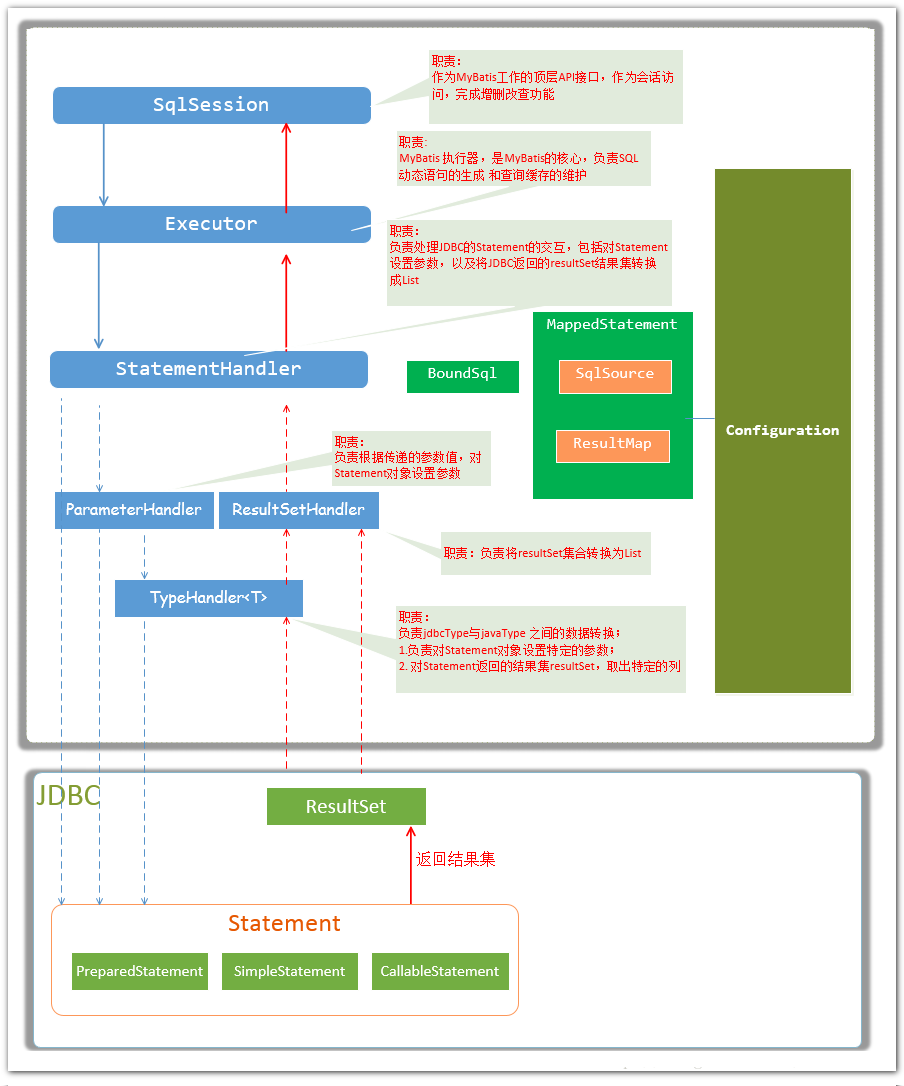
\includegraphics[scale=0.4]{./images/0017.png}
    \caption{MyBatis中SQL语句的执行流程}
\end{figure}

\subsection{MyBatis缓存}
\subsubsection{一级缓存}
一级缓存是sqlSession级别的缓存。在操作数据库时需要构造sqlSession对象,在对象中有一个HashMap用于存储缓存数据。不同的sqlSession之间的缓存数据区域是互不影响相互独立的。也就是他只能作用在同一个sqlSession中,不同的sqlSession中的缓存是互相不能读取的。Mybatis一级缓存默认开启。\\
这个HashMap的key是以查询的sql语句为基础的拼接出的一个字符串组成的。\\
用户发起查询请求,查找某条数据,sqlSession先去缓存中查找,是否有该数据,如果有从缓存中读取。如果没有,从数据库中查询,并将查询到的数据放入一级缓存,供下次查找使用。当sqlSession执行了commit操作(增删改),一级缓存会清空,以使得缓存的都是最新的数据,避免脏读。\\
如果commit不清空缓存,会有以下场景:A查询了某商品库存为10件,并将10件库存的数据存入缓存中,之后被客户买走了10件,数据被delete了,但是下次查询这件商品时,并不从数据库中查询,而是从缓存中查询,就会出现错误。\\
实际应用中,如果将Spring和Mybatis进行整合,事务控制发生在service中。service开始执行时创建sqlSession对象,结束时关闭sqlSession,如果刚刚产生了一级缓存的话,也会随着sqlSession而销毁。所以两次调用相同的service查询相同的信息,不会走一级缓存的。
\subsubsection{二级缓存}
二级缓存默认不开启。需要在MyBatis的配置文件中加入:
\begin{minted}{xml}
    <settings>
        <!-- 开启二级缓存 -->
        <setting name="cacheEnabled" value="true"/>
    </settings>
\end{minted}
以及在需要打开二级缓存的mapper.xml文件中加入cache标签:
\begin{minted}{xml}
    <cache/>
\end{minted}
同时也要让使用二级缓存的POJO类实现Serializable接口,例如:
\begin{minted}{java}
    public class User implements Serializable {
        ...
    }
\end{minted}
二级缓存是mapper级别的缓存,多个SqlSession去操作同一个Mapper的sql语句,多个SqlSession可以共用二级缓存,二级缓存是跨SqlSession的。每一个namespace的mapper都有一个自己的二级缓存区域,如果两个mapper有相同的namespace,那么这两个mapper查询到的数据将会存储在相同的二级缓存区域中。\\
前面我们说到,Spring和MyBatis整合时,每次查询之后都要进行关闭sqlSession,关闭之后数据被清空。所以spring整合之后,如果没有事务,一级缓存是没有意义的。那么如果开启二级缓存,关闭sqlsession后,会把该sqlsession一级缓存中的数据添加到namespace的二级缓存中。这样,缓存在sqlsession关闭之后依然存在。同样,commit操作也会清空该mapper下的二级缓存。\\
二级缓存是建立在同一个namespace下的,如果对表的操作查询可能有多个namespace,那么得到的数据就是错误的。\\
例如,订单和订单详情,orderMapper、orderDetailMapper。在查询订单详情时我们需要把订单信息也查询出来,那么这个订单详情的信息被二级缓存在orderDetailMapper的namespace中,这个时候有人要修改订单的基本信息,那就是在orderMapper的namespace下修改,他是不会影响到orderDetailMapper的缓存的,那么你再次查找订单详情时,拿到的是缓存的数据,这个数据其实已经是过时的。\\
因此,使用二级缓存需要注意以下两点:
\begin{enumerate}
    \item 对该表的操作与查询都在同一个namespace下,其他的namespace如果有操作,就会发生数据的脏读。
    \item 对关联表的查询,关联的所有表的操作都必须在同一个namespace。
\end{enumerate}

\subsection{MyBatis的一对一、一对多关联查询}
使用association标签设置一对一关联映射,使用collection标签设置一对多关联映射。
\begin{minted}{xml}
    <mapper namespace="com.lcb.mapping.userMapper">
        <!-- association  一对一关联查询 -->
        <select id="getClass" parameterType="int" resultMap="ClassesResultMap">
            select * from class c,teacher t where c.teacher_id=t.t_id and c.c_id=#{id}
        </select>

        <resultMap type="com.lcb.user.Classes" id="ClassesResultMap">
            <!-- 实体类的字段名和数据表的字段名映射 -->
            <id property="id" column="c_id"/>
            <result property="name" column="c_name"/>
            <association property="teacher" javaType="com.lcb.user.Teacher">
                <id property="id" column="t_id"/>
                <result property="name" column="t_name"/>
            </association>
        </resultMap>

        <!-- collection  一对多关联查询 -->
        <select id="getClass2" parameterType="int" resultMap="ClassesResultMap2">
            select * from class c,teacher t,student s where c.teacher_id=t.t_id and c.c_id=s.class_id and c.c_id=#{id}
        </select>

        <resultMap type="com.lcb.user.Classes" id="ClassesResultMap2">
            <id property="id" column="c_id"/>
            <result property="name" column="c_name"/>
            <association property="teacher" javaType="com.lcb.user.Teacher">
                <id property="id" column="t_id"/>
                <result property="name" column="t_name"/>
            </association>

            <collection property="student" ofType="com.lcb.user.Student">
                <id property="id" column="s_id"/>
                <result property="name" column="s_name"/>
            </collection>
        </resultMap>
    </mapper>
\end{minted}

\end{document}
